\section {Re'tele de tip ANFIS}

\paragraph{}

Vom continua lucrarea prin a prezenta modelul de re'tele ANFIS \cite{anfis}. Acesta introduce conceptul de sistem de inferen't;a fuzzy bazat pe o re'tea adaptiv;a, care poate construi o mul'time de reguli fuzzy \textit{if-then} cu func'tiile de apartenen't;a potrivita a'sa 'inc'at s;a genereze perechi intrare-ie'sire pentru datele oferite. 
\par
\subsection{Reguli fuzzy if-then}
\paragraph{}
Regulile fuzzy if-then (sau expresiile fuzzy condi'tionale) sunt de forma \textit{IF A THEN B}, unde A 'si B sunt etichete ale unor mul'timi fuzzy, caracterizate de c;atre func'tiile lor de apartenen't;a. Datorit;a formei lor compacte, ele sunt folosite pentru a modela moduri imprecise de g'andire care joac;a un rol esen'tial 'in abilitatea uman;a de a lua decizii 'intr-un mediu incert 'si imprecis.
Jang ofer;a un exemplu clar 'si concis pentru a ilustra o regul;a fuzzy if-then: \\
\begin{center}\textit{If pressure is high, then volume is small} \cite{anfis} \end{center}
unde \textit{pressure} 'si \textit{volume} sunt variabile lingvistice, iar \textit{high} 'si \textit{small} sunt valori lingvistice caracterizate de c;atre func'tiile de apartenen't;a.
\par
Un alt fel de reguli fuzzy if-then sunt cele de tip Takagi-Sugeno \cite{takagisugeno} de forma: \\
\begin{center}$if\ x_{1} = small\ and\ x_{2} = big\ then\ y = x_{1} + x_{2}$ \end{center}
unde, din nou, small 'si high sunt valori lingvistice caracterizate de c;atre func'tiile lor de apartenen't;a. Diferen'ta apare 'in partea consecvent;a, rezultatul fiind de aceast;a dat;a o ecua'tie non-fuzzy ce depinde de variabilele $x_{1}$ 'si $x_{2}$. 
\par
Definim 'in continuare un sistem de inferen't;a fuzzy (cunoscut 'si ca model fuzzy sau controller fuzzy c'and este folosit pe post de controller). Un sistem de inferen't;a fuzzy este compus din cinci unit;a'ti func'tionale:
\begin{itemize}
\item o baz;a de reguli ce con'tine reguli fuzzy if-then;
\item o baz;a de date ce define'ste func'tiile de apartenen't;a ale mul'timilor fuzzy folosite 'in regulile fuzzy;
\item o unitate de decizie care execut;a opera'tiile de inferen't;a peste reguli;
\item o interfa't;a de fuzzificare ce transform;a intr;arile crisp 'in grade de apartenen't;a la valori lingvistice;
\item o interfa't;a de defuzzificare ce transform;a rezultatele fuzzy ale inferen'tei 'inapoi 'in date crisp
\end{itemize}
De obicei baza de reguli si baza de date sunt grupate 'impreun;a sub denumirea de "baz;a de cunoa'stere".
\par \newpage
Pa'sii inferen'tei fuzzy sunt urm;atorii:
\begin{enumerate}
\item Variabilele de intrare sunt comparate prin func'tiile de apartenen't;a 'in partea de premis;a pentru a li se oferi valorile de apartenen't;a (fuzzificare)
\item Valorile de apartenen't;a sunt combinate pentru a ob'tine ponderea fiec;arei reguli (combinarea are loc printr-un operator T-normat\footnote{Un operator T-normat este o func'tie $T: [0,1] \times [0, 1] \to [0, 1]$ care satisface condi'tiile: \\
Comutativitate: $T(a, b) = T(b, a)$ \\
Monotonie: $T(a, b) \leq T(c, d)$ dac;a $a \leq c$ 'si $b \leq d$ \\
Asociativitate: $T(a, T(b, c)) = T(T(a, b), c)$ \\
Num;arul 1 are comportamentul elementului identitate: $T(a, 1) = a$}, de obicei multiplicare)
\item Este generat consecventul fiec;arei reguli (fie el fuzzy sau crisp), 'in func'tie de ponderi
\item Consecven'tii sunt agrega'ti pentru a produce o ie'sire crisp (defuzzificare)
\end{enumerate}
\par
\subsection{Re'tele adaptive}
\par \paragraph{}
Re'telele adaptive sunt un superset al mul'timii re'telelor \textit{feedforward} cu capacitate de 'inv;a'tare supervizat;a. Dup;a cum numele sugereaz;a, re'telele adaptive sunt structuri ce con'tin noduri 'si leg;aturi direc'tionale pentru interconectarea nodurilor, rezult'and 'intr-o re'tea. Cel pu'tin o parte dintre noduri sunt adaptive, ceea ce 'inseamn;a c;a ie'sirile acestora depind de parametrii pe care 'ii primesc, iar regulile de 'inv;a'tare dicteaz;a cum ace'sti parametri se schimb;a pentru a optimiza o func'tie de eroare.
\par
Regula de 'inv;a'tare de baz;a a re'telelor adaptive se bazeaz;a pe pe gradientul descendent 'si pe regula 'inl;an'tuirii. Dar, deoarece metoda gradientului descendent este cunoscut;a ca fiind foarte lent;a 'si risc;a s;a ajung;a blocat;a 'in minime locale, arhitectura ANFIS propune un algoritm de 'inv;a'tare hibrid, care este mai rapid, 'si care func'tioneaz;a at'at 'in mod \textit{batch} (off-line) c'at 'si \textit{pattern} (on-line).
\begin{figure}[!htbp]
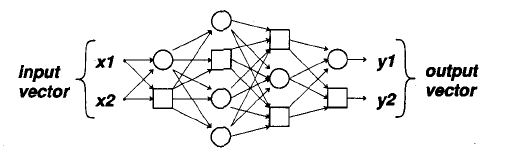
\includegraphics[width=\textwidth]{adaptive_net}
\caption {Arhitectura unei re'tele adaptive cu dou;a intr;ari 'si dou;a ie'siri}
\end{figure}
\newpage

\paragraph{}

A'sa cum am enun'tat 'inainte, o re'tea adaptiv;a este o re'tea multi-strat feedforward 'in care fiecare nod evalueaz;a o anumit;a func'tie (numit;a 'si func'tie de nod) pe semnalele de intrare, 'si, 'in plus, fiecare nod are 'si o mul'time de parametri. Formulele pentru func'tiile de nod pot varia de la nod la nod, iar alegerea lor depinde de func'tia pe care re'teaua trebuie s;a o modeleze. O particularitate important;a este c;a leg;aturile dintre noduri indic;a doar direc'tia pe care o parcurge semnalul;\ nu exist;a niciun fel de ponderi asociate leg;aturilor dintre noduri.
\par
Figura 7.1 ilustreaz;a o posibil;a configura'tie a unei re'tele cu doi parametri de intrare 'si doi parametri de ie'sire. Pentru a diferen'tia tipurile de noduri dintr-o re'tea adaptiv;a, sunt folosite noduri 'in forma rotund;a pentru a indica un nod fixat, ce nu prime'ste parametri, 'si noduri 'in forma p;atrat;a pentru a indica noduri adaptive, ce primesc parametri. Mul'timea parametrilor unei re'tele adaptive este reuniunea tuturor mul'timilor de parametri ale tuturor nodurilor adaptive. Pentru a ob'tine o modelare a unei func'tii dup;a intr;ari 'si ie'siri, ace'sti parametri sunt actualiza'ti folosind datele de antrenare 'si o regul;a de 'inv;a'tare bazat;a pe gradient prezentat;a 'in continuare.
\par
Fie o re'tea adaptiv;a cu $L$ straturi 'si cu al k-lea strat av'and $\#(k)$ noduri. Not;am al i-lea nod de pe stratul k cu $(k, i)$ 'si func'tia de nod cu $O_{i}^{k}$. Din moment ce semnalul de ie'sire al unui nod depinde de semnalele de intrare 'si de parametrii s;ai, avem
\begin{equation}
O_{i}^{k} = O_{i}^{k} (O_{1}^{k-1}, ... , O_{\#(k-1)}^{k-1}, a, b, c, ...)
\end{equation}
unde $a, b, c, ...$ sunt parametrii corespunz;atori acestui nod. (Not;a: am folosit $O_{i}^{k}$ at'at pentru a ne referi la semnalul de ie'sire al nodului c'at 'si la func'tia sa.)
\par
Av'and un set de date antrenare cu P intr;ari, putem defini m;asura de eroare pentru a $p$-a intrare ($1 \leq p \leq P$) din setul de date de antrenare ca fiind suma p;atratelor erorilor:
\begin{equation}
E_{p} = \displaystyle \sum_{m = 1}^{\#(L)} (T_{m, p} - O_{m, p}^{L})^{2}
\end{equation}
unde $T_{m, p}$ este a $m$-a component;a a celui de al $p$-lea vector 'tint;a de rezultate, iar $O_{m, p}^{L}$ este a $m$-a component;a a vectorului real de rezultate, produs prin prezentarea celui de-al $p$-lea vector de intr;ari.
\par
Prin urmare, m;asura total;a a erorii este
\begin{equation}
E = \displaystyle \sum_{p=1}^{P} E_{p}
\end{equation}

\paragraph{}
Pentru a ob'tine o procedur;a de 'inv;a'tare care s;a implementeze gradientul descendent 'in $E$ peste spa'tiul parametrilor, avem nevoie 'in primul r'and de rata de eroare $\frac {\partial E_{p}} {\partial O}$ pentru al $p$-lea punct din datele de antrenare 'si pentru fiecare ie'sire de nod $O$. Rata de eroare pentru nodul ($L, i$) devine (ob'tinut;a din 7.2)
\begin{equation}
\frac {\partial E_{p}} {\partial O_{i, p}^{k}} = -2(T_{i, p} - O_{i, p}^{L})
\end{equation}
Pentru nodul intern de la ($k, i$), rata de eroare poate fi derivat;a folosind regula 'inl;an'tuirii \footnote{Regula 'inl;an'tuirii este definit;a prin $\frac{dz}{dx} = \frac{dz}{dy} \cdot \frac{dy}{dx}$;\ i.e. av'and trei variabile $x, y, z$, cu $z$ dependent;a de $y$, iar $y$ dependent;a de $x$ astfel 'inc'at $y$ 'si $z$ sunt variabile dependente, atunci $z$, prin intermediul lui $y$ depinde de $x$.}
\begin{equation}
\frac {\partial E_{p}} {\partial O_{i, p}^{k}} = \displaystyle \sum_{m = 1}^{\#(k+1)} \frac {\partial E_{p}} {\partial O_{m, p}^{k+1}} \cdot \frac {\partial O_{m, p}^{k+1}} {\partial O_{i, p}^{k}}
\end{equation}
unde $1 \leq k \leq L-1$. Deci, rata de eroare a unui nod intern poate fi explicitat;a sub form;a de combina'tie liniar;a a ratelor de eroare ale nodurilor de pe stratul urm;ator. Prin urmare, pentru to'ti $1 \leq k \leq L$ 'si $1 \leq i \leq \#(k)$ putem g;asi $\frac {\partial E_{p}} {\partial O_{i, p}^{k}}$ conform cu 7.4 'si 7.5.
\par
S;a presupunem $\alpha$ un parametru al re'telei adaptive. Avem a'sadar
\begin{equation}
\frac {\partial E_{p}} {\partial \alpha} = \displaystyle \sum_{O^{*} \in S} \frac {\partial E_{p}} {\partial O^{*}} \cdot \frac {\partial O^{*}} {\partial \alpha}
\end{equation}
unde S este mul'timea nodurilor ale c;aror ie'siri depind de $\alpha$. Derivata m;asurii totale a erorii $E$ 'in raport cu $\alpha$ devine:
\begin{equation}
\frac {\partial E_{p}} {\partial \alpha} = \displaystyle \sum_{p = 1}^{P} \frac {\partial E_{p}} {\partial \alpha}
\end{equation}
\par
Formula de actualizare pentru parametrul generic $\alpha$ este:
\begin{equation}
\Delta \alpha = - \eta \frac {\partial E} {\partial \alpha}
\end{equation}
unde $\eta$ este rata de 'inv;a'tare care poate fi exprimat;a 'si ca:
\begin{equation}
\eta = - \frac {k} {\sqrt {\displaystyle \sum_{\alpha} \Big(\frac {\partial E} {\partial \alpha}\Big)^{2}}}
\end{equation}
unde $k$ este dimensiunea pasului, adic;a lungimea fiec;arei tranzi'tii a gradientului 'in spa'tiul parametrilor. De obicei, valorea lui $k$ poate fi schimbat;a pentru a varia viteza de convergen't;a.
\par
Exist;a dou;a metode de 'inv;a'tare pentru re'telele adaptive. Prin 'inv;a'tarea de tip batch (off-line) formula de actualizare a parametrului $\alpha$ este bazat;a pe (7.7), iar ac'tiunea de actualizare are loc doar atunci c'and intreg setul de date de antrenare a fost parcurs, i.e. dup;a o epoc;a.
\par
'In contrast, dac;a dorim ca parametrii s;a fie actualiza'ti imediat cum o pereche intrare-ie'sire i-a fost prezentat;a re'telei, atunci formula de 'inv;a'tare este bazat;a pe (7.6), 'si ne vom referi la ea ca 'inv;a'tare pattern (sau on-line). 'In continuare, prezent;am o derivare a unei reguli hibride 'si rapide sub ambele forme: off-line si on-line.
\par
\subsection{Regula de 'inv;a'tare hibrid;a off-line}
\paragraph{}

Regula de 'inv;a'tare hibrid;a off-line propune o combina'tie 'intre metoda gradientului 'si metod;a estim;arii p;atratelor minime pentru a identifica parametrii. De'si s-ar putea aplica metoda gradientului, aceasta este lent;a 'si exist;a posibilitatea ca ea s;a r;aman'a blocat;a 'in minime locale.
\par
S;a presupunem c;a re'teaua adaptiv;a pe care vom aplica regula are o singur;a ie'sire:
\begin{equation}
ie'sire = F(\overrightarrow{I}, S)
\end{equation}
unde $\overrightarrow{I}$ este mul'timea variabilelor de intrare 'si $S$ este mul'timea parametrilor. Dac;a exist;a o func'tie $H$ astfel 'inc'at compunerea $H \circ F$ este liniar;a 'in unele elemente din $S$, atunci aceste elemente pot fi identificate prin metoda p;atratelor minime. Formal, daca descompunem $S$ 'in
\begin{equation}
S = S_{1} \oplus S_{2}
\end{equation}
unde $\oplus$ reprezint;a 'insumarea direct;a, astfel 'inc'at $H \circ F$ este liniar;a 'in $S_{2}$, atunci aplic'and $H$ pe (7.10) avem
\begin{equation}
H(ie'sire) = H \circ F(\overrightarrow{I}, S)
\end{equation}
care este liniar;a 'in $S_{2}$. Date fiind valorile elementelor din $S_{1}$ putem introduce datele de antrenare $P$ 'in (7.12) ob'tin'and o ecua'tie matriceal;a:
\begin{equation}
AX = B
\end{equation}
unde $X$ este un vector de necunoscute ale c;arui elemente sunt parametri 'in $S_{2}$. Fie $|S_{2}| = M$, atunci dimensiunile lui $A, X$ 'si $B$ sunt $P \times M, M \times 1$, respectiv $P \times 1$. Din moment de $P$ este, de obicei, mai mare dec'at $M$ (num;arul de puncte de date de antrenare este mai mare dec'at num;arul de parametri liniari), aceasta este o problem;a compatibil nedeterminat;a, 'si, 'in general, nu exist;a o solu'tie exact;a pentru (7.13). Prin urmare, o estimare a celor mai mici p;atrate ale lui $X$, $X^{*}$, este c;autat;a pentru a minimiza eroarea p;atrat;a $||AX - B||^{2}$. Aceasta este o problem;a standard ce st;a la baza regresiei liniare, filtr;arii adaptive 'si proces;arii de semnale. Cea mai cunoscut;a formul;a pentru $X^{*}$ se folose'ste de pseudo-inversa lui $X$:
\begin{equation}
X^{*} = (A^{T}A)^{-1}A^{T}B
\end{equation}
unde $A^{T}$ este transpusa lui $A$, iar $(A^{T}A)^{-1}A^{T}$ este pseudo-transpusa lui $A$, dac;a $A$ este non-singular;a. De'si (7.14) are o nota'tie clar;a, 'si ea este u'sor de construit intuitiv, calcularea inversei este un proces foarte costisitor din punct de vedere computa'tional. Mai mult, ecua'tia nu este bine definit;a dac;a $A^{T}A$ este singular;a. Prin urmare, \cite{anfis} prezint;a o metod;a secven'tial;a de a calcula estimarea celor mai mici p;atrate ale lui $X$. Aceast;a metod;a secven'tial;a este eficient;a, 'si poate fi modificat;a 'intr-o variant;a on-line.
\par
Fie al $i$-lea vector r'and din matricea $A$ definit;a 'in (7.13) notat cu $a_{i}^{T}$, 'si al $i$-lea element din $B$ notat cu $b_{i}^{T}$. Atunci $X$ poate fi calculat iterativ folosind formule secven'tiale adoptate din literatur;a:
\begin{equation}
\begin{aligned}
X_{i+1} = X_{i} + S_{i+1}a_{i+1}(b_{i+1}^{T} - a_{i+1}^{T}X_{i}) \\
S_{i+1} = S_{i} - \frac {S_{i}a_{i+1}a_{i+1}^{T}S_{i}} {1 + a_{i+1}^{T}S_{i}a_{i+1}},\  i = 0, 1, ..., P-1
\end{aligned}
\end{equation}
unde $S_{i}$ este matricea de covarian't;a 'si estimarea celor mai mici p;atrate este egal;a cu $X_{P}$. Condi'tiile ini'tiale pentru a aplica \textit{bootstrapping}\footnote {Bootstrapping este o metod;a de inferen't;a statistic;a bazat;a pe folosirea unei singure e'santion;ari 'si 'inlocuirea  aleatorie a unor puncte din datele e'santionate cu alte puncte din acela'si e'santion, 'in mod repetat.} sunt $X_{0} = 0$ 'si $S_{0} = \gamma I$, unde $\gamma$ este un num;ar pozitiv mare, iar $I$ este matricea identitate de dimensiune $M \times M$.
Atunci c'and re'teaua adaptiv;a are mai multe ie;siri, ($ie'sire$ din (7.10) este un vector coloan;a), atunci (7.15) r;am'ane valabil;a, dar $b_{i}^{T}$ devine al $i$-lea r'and din $B$.
\par
Putem acum s;a combin;am metoda gradientului 'si metoda estim;arii p;atratelor minime pentru a actualiza parametrii dintr-o re'tea adaptiv;a. Fiecare epoc;a a acestei proceduri hibride de 'inv;a'tare este compus;a dintr-o propagare 'inainte 'si o propagare 'inapoi. 'In propagarea 'inainte oferim datele de intrare 'si semnalele func'tionale, iar acestea se propag;a 'inainte pentru a calcula ie'sirea fiec;arui nod p'an;a se ob'tin matricele $A$ 'si $B$ din (7.13), iar parametrii din $S_{2}$ sunt identifica'ti dup;a formula secven'tial;a a celor mai mici p;atrate din (7.15). Dup;a ce au fost identifica'ti parametrii din $S_{2}$, semnalele func'tionale continu;a s;a se propage 'inainte p'an;a c'and m;asura erorii este calculat;a. 'In propagarea 'inapoi ratele de eroare (derivatele m;asurii erorii 'in raport cu fiecare ie'sire de nod) se propag;a dinspre ie'siri c;atre intr;ari, iar parametrii din $S_{1}$ sunt actualiza'ti dup;a metoda gradientului din (7.9).
\par
Pentru valori fixate date parametrilor din $S_{1}$, este garantat c;a valorile parametrilor din $S_{2}$ sunt puncte globale de optim din spa'tiul parametrilor lui $S_{2}$ datorit;a alegerii m;asurii de eroare a p;atratelor. Nu numai c;a aceast;a regul;a hibrid;a de 'inv;a'tare descre'ste dimensiunea spa'tiului de c;autare din metoda gradientului, dar, 'in general, va avea un timp de convergen't;a substan'tial mai mic.
\par
Lu'and ca exemplu o re'tea neuronal;a cu propagare 'in spate 'si func'tia de activare sigmoid, dac;a ea are $p$ unit;a'ti de ie'sire, atunci $ie'sire$ din (7.10) este un vector coloan;a. Fie $H(\cdot)$ inversa func'tiei sigmoid:
\begin{equation}
H(x) = ln (\frac {x} {1-x})
\end{equation}
atunci (7.12) devine o func'tie liniar;a astfel 'inc'at fiecare element din $H(ie'sire)$ este o combina'tie liniar;a 'intre parametrii (ponderi 'si praguri) ce 'tin de stratul cu num;arul 2. 'In alte cuvinte, \\
$S_{1}$ =  ponderile 'si pragurile stratului ascuns \\
$S_{2}$ = ponderile 'si pragurile stratului de ie'sire \\
Prin urmare, putem aplica regula de 'inv;a'tare back-propagation pentru a regla parametrii stratului ascuns, 'si parametrii stratului de ie'sire pot fi identifica'ti de c;atre metoda celor mai mici p;atrate. Trebuie totu'si notat c;a folosind metoda celor mai mici p;atrate peste datele transformate de c;atre $H(\cdot)$ , parametrii ob'tinu'ti sunt optimi 'in func'tie de m;asura erorii cu eroarea la p;atrat, 'in loc de cea original;a. De obicei, acest lucru nu ridic;a o problem;a real;a c'at timp $H(\cdot)$ este monoton cresc;atoare.
\par

\subsection{Regula de 'inv;a'tare hibrid;a on-line}
\paragraph{}

Dac;a parametrii sunt actualiza'ti dup;a fiecare prezentare a datelorf atunci avem de a face cu paradigma 'inv;a'tarii on-line. Aceast;a paradigm;a este crucial;a pentru identificarea parametrilor 'in sistemele cu caracteristici care sunt 'in schimbare. Pentru a modifica regula off-line 'intr-o variant;a off-line este suficient s;a observ;am c;a gradientul descendent trebuie s;a fie bazat pe $E_{p}$ (vezi (7.6)) 'in loc de $E$. Formal, aceasta nu este o procedur;a 'in gradient adev;arat;a de minimizare a lui $E$, dar ea o va aproxima dac;a rata de 'inv;a'tare este mic;a.
\par
Pentru ca formula secven'tial;a a celor mai mici p;atrate s;a poat;a fi adaptat;a la caracteristicile variabile 'in func'tie de timp ale datelor de intrare, este necesar ca perechile de date vechi s;a aib;a o pondere din ce 'in ce mai mic;a odat;a ce apar date noi. 'Inc;a odat;a, aceast;a problem;a este studiat;a 'si rezolvat;a 'in literatura controlului adaptiv. O metod;a este formularea m;asurii erorii p;atratelor 'intr-o variant;a ponderat;a, unde datele mai vechi primesc factori mai mici de pondere fa't;a de cele mai noi. Acest lucru este echivalent cu ad;augarea unui factor de uitare $\lambda$ 'in formula secven'tial;a original;a:
\begin{equation}
\begin{aligned}
X_{i+1} = X_{i} + S_{i+1}a_{i+1}(b_{i+1}^{T} - a_{i+1}^{T}X_{i}) \\
S_{i+1} = \frac {1}{\lambda} [S_{i} - \frac {S_{i}a_{i+1}a_{i+1}^{T}S_{i}} {\lambda + a_{i+1}^{T}S_{i}a_{i+1}}],\  i = 0, 1, ..., P-1
\end{aligned}
\end{equation}
unde $\lambda$ este 'intre $0$ 'si $1$. Cu c'at $\lambda$ descre'ste, cu at'at mai mult se observ;a efectele sl;abirii datelor vechi. Dar, uneori, un $\lambda$ mic poate duce la instabilitate numeric;a, deci ar trebui evitat.

\newpage
\subsection{Arhitectura ANFIS}
\paragraph{}

'Stiind acum defini'tia, arhitectura 'si regulile de 'inv;a'tare ale unei re'tele adaptive, putem deduce faptul c;a func'tional, nu exist;a aproape nicio constr'angere asupra func'tiilor de nod 'in afar;a de diferen'tiabilitatea pe por'tiuni\footnote{O func'tie $f$ se nume'ste diferen'tiabil;a pe por'tiuni dac;a: \\
$f$ este definit;a pe por'tiuni (exist;a mai multe sub-func'tii ale lui $f$, fiecare aplicat;a pentru un anumit interval din domeniul lui $f$) \\
Pentru fiecare por'tiune a lui $f$, subfunc'tia corespunz;atoare acelei por'tiuni este diferen'tiabil;a de-a lungul 'intregului subdomeniu}, iar structural, singura limitare a configura'tiei re'telei este c;a aceasta trebuie sa fie de tip feedforward. Datorit;a acestor restric'tii minimale, observ;am c;a aplica'tiile re'telelor adaptive sunt vaste 'si imediate 'in diverse domenii. Vom prezenta 'in continuare o arhitectur;a de re'tele care sunt echivalente func'tional cu un sistem de inferen't;a fuzzy. Vom descrie o metod;a de descompunere a mul'timii parametrilor pentru a aplica regula de 'inv;a'tare hibrid;a.
\par
S;a presupunem un sistem de inferen't;a fuzzy cu dou'a variabile de intrare $x, y$ 'si una de ie'sire $z$. Presupunem c;a baza de reguli con'tine dou'a reguli fuzzy if-then de tip Takagi-Sugeno:
\begin{enumerate}
\item if $x$ is $A_{1}$ and $y$ is $B_{1}$ then $f_{1} = p_{1}x + q_{1}y + r_{1}$
\item if $x$ is $A_{2}$ and $y$ is $B_{2}$ then $f_{2} = p_{2}x + q_{2}y + r_{2}$
\end{enumerate}
\begin{figure}[!htbp]
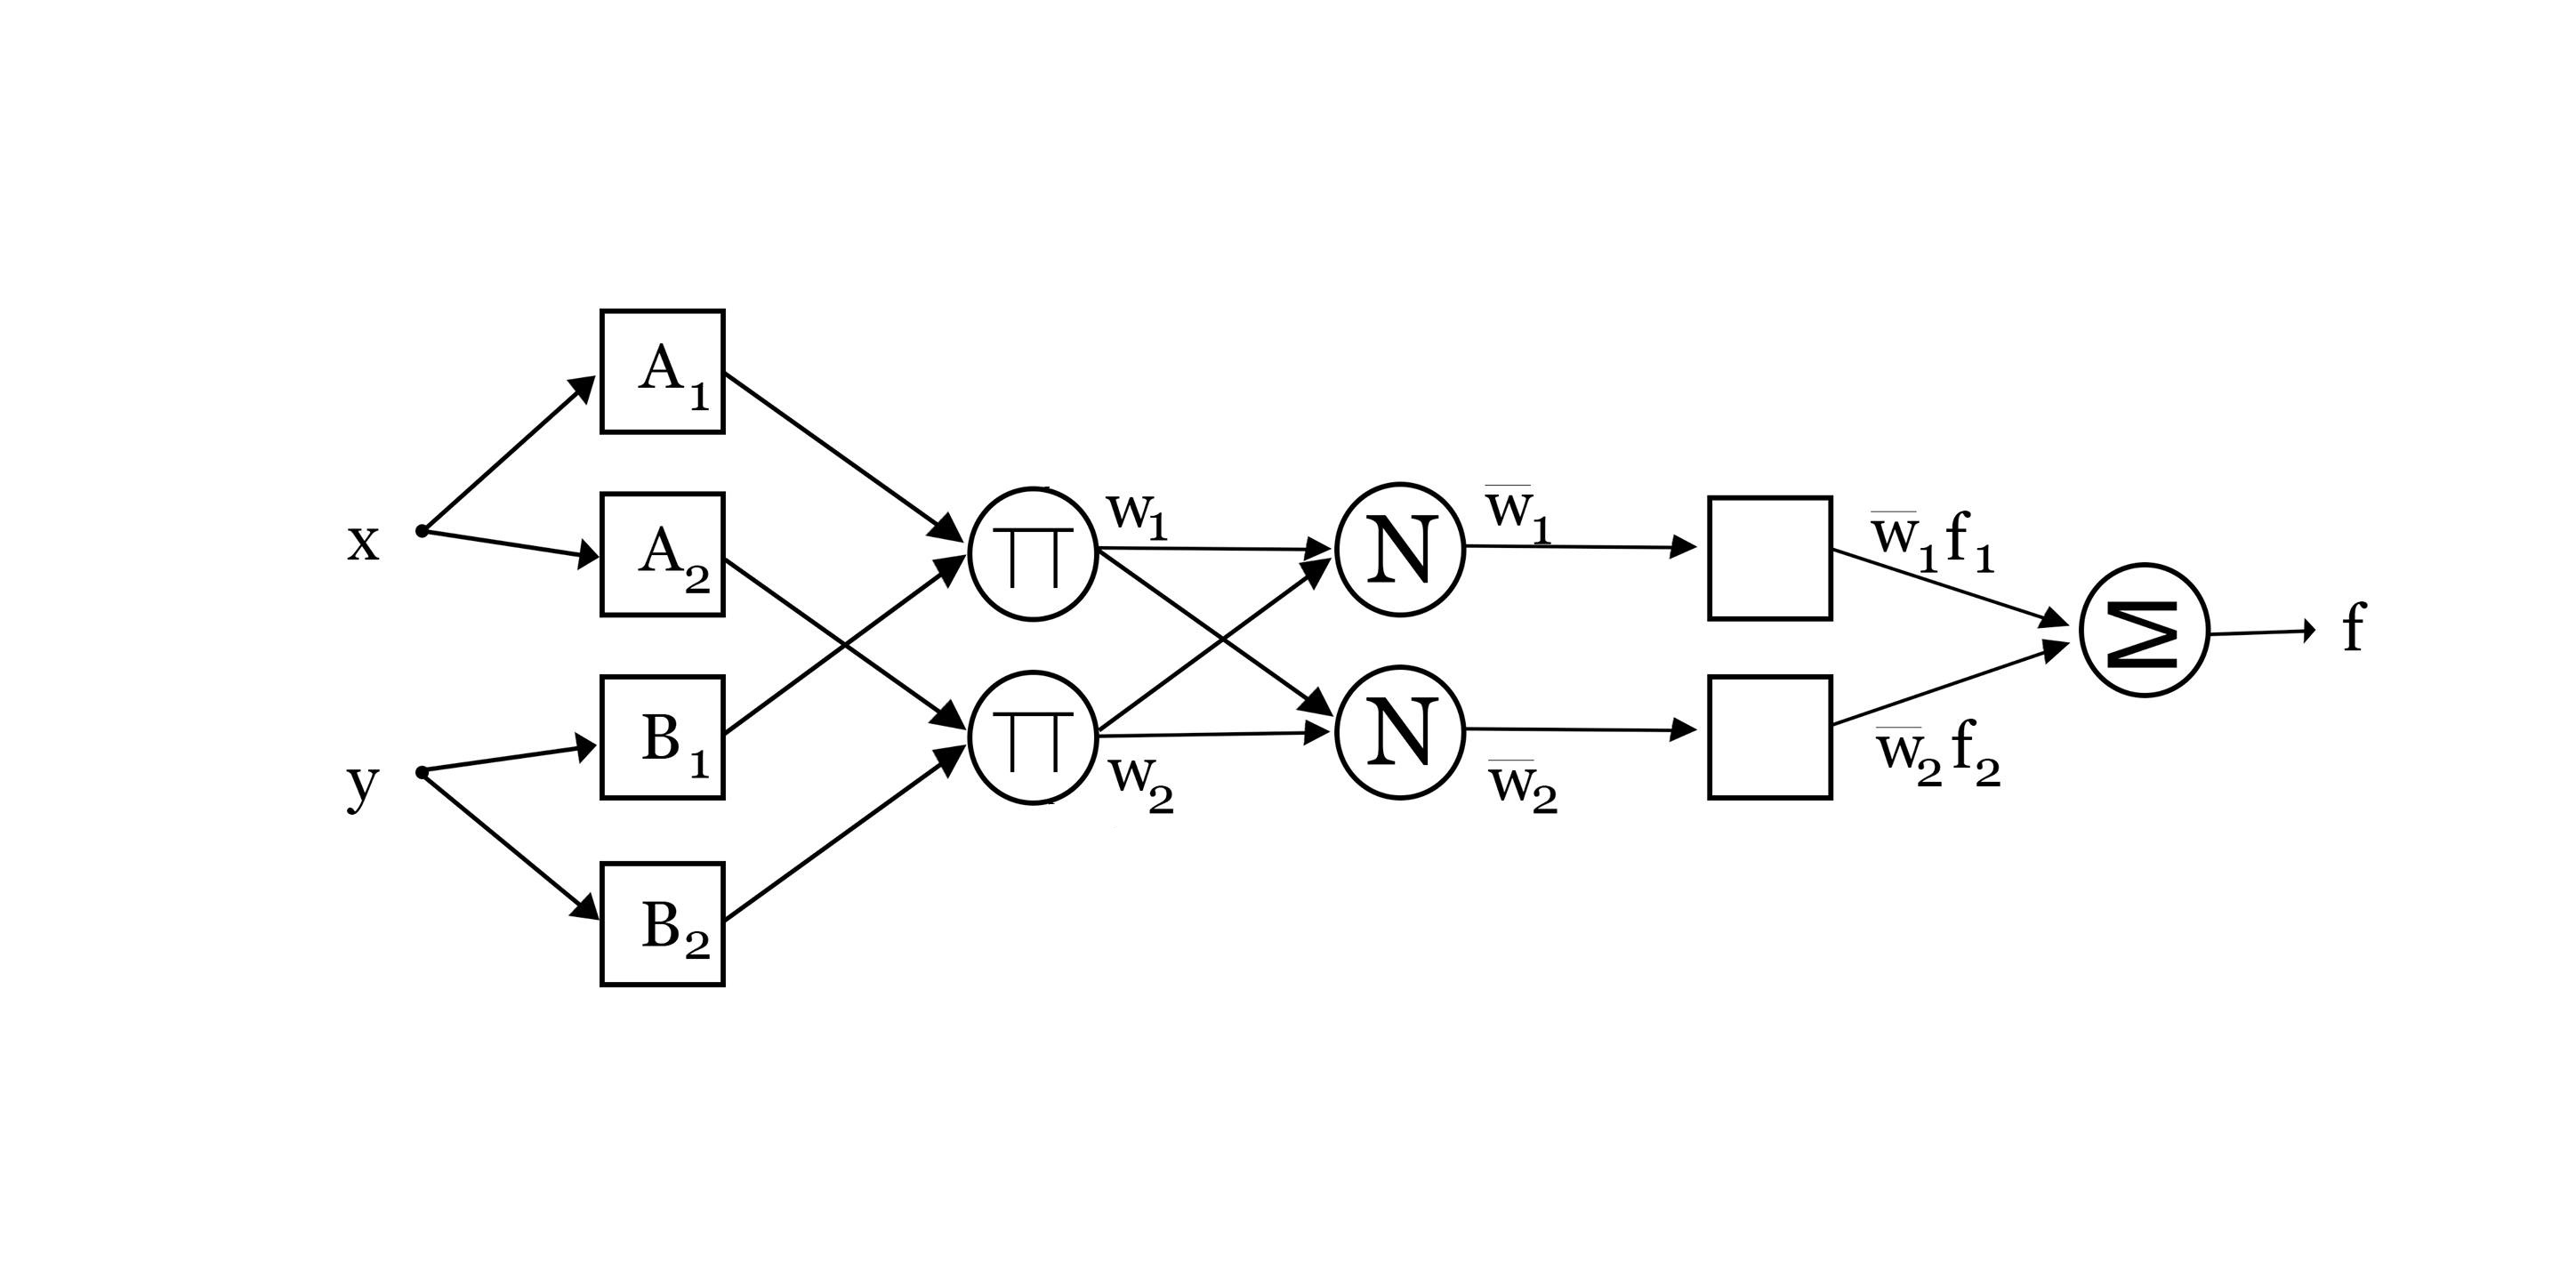
\includegraphics[width=\textwidth]{anfisarch}
\caption{Arhitectur;a ANFIS pentru dou;a reguli fuzzy if-then Takagi-Sugeno.}
\end{figure}
\newpage
\paragraph{}
Toate func'tiile de node apar'tin uneia din familiile de func'tii definite 'in continuare, 'in func'tie de strat:
\begin{enumerate}
\item [Stratul 1:] Fiecare nod $i$ din acest strat este un nod adaptiv cu o func'tie de nod 
\begin {equation}
O_{i}^{1} = \mu_{A_{i}}(x)
\end{equation}
unde $x$ este intrarea pentru nodul $i$, 'si $A_{i}$ este eticheta 'in limbaj natural (i.e. mic, mare, etc.) asociat;a acestei func'tii de nod. Altfel spus, $O_{i}^{1}$ este func'tia de apartenen't;a a lui $A_{i}$, specific'and gradul cu care un $x$ dat satisface cuantificatorul $A_{i}$. De obicei, se alege $\mu_{A_{i}}(x)$ astfel 'inc'at s;a fie gaussian;a cu maximul egal cu $1$ 'si minimul egal cu $0$, cu formele:
\begin{equation}
\mu_{A_{i}}(x) = \frac {1} {1 + [(\frac {x - c_{i}} {a_{i}})^2]b_{i}}
\end{equation}
sau
\begin{equation}
\mu_{A_{i}}(x) = exp[- (\frac {x-c_{i}} {a_{i}} )^{2}]
\end{equation}
unde \{$a_{i}, b_{i}, c_{i}$\} este mul'timea de parametri. 'In func'tie de schimb;arile parametrilor, func'tiile gaussiene variaz;a corespunz;ator, ar;at'and astfel diefirte forme de func'tii de apartenen't;a peste eticheta 'in limbaj natural $A_{i}$. De fapt, orice func'tii continue 'si diferen'tiabile pe por'tiuni, cum ar fi func'tiile de apartenen't;a trapezoidale sau triunghiulare, sunt candida'ti buni pentru acest strat. Parametrii acestui strat se mai numesc 'si parametri de premise.
\item [Stratul 2:] Fiecare nod din acest strat este un nod fix (i.e. nu are parametri) etichetat cu $\Pi$, care 'inmul'te'ste semnalele primite 'si trimite produsul acestora. De exemplu,
\begin{equation}
w_{i} = \mu_{A_{i}}(x) \times \mu_{B_{i}}(y),\ i = 1,2.
\end{equation}
Fiecare ie'sire de nod reprezint;a puterea de "aprindere" a regulii. Mai mult, orice al'ti operatori T-norma'ti care calculeaz;a un "'SI" generalizat pot fi folosite ca func'tii de nod pe acest strat.
\item [Stratul 3:] Fiecare nod de pe acest strat este un nod fix etichetat cu "N". Cel de-al $i$-lea nod calculeaz;a raportul puterii de "aprindere" a celei de a $i$-a regul;a la suma tuturor puterilor de "aprindere" ale regulilor.
\begin{equation}
\bar w_{i} = \frac {w_{i}} {w_{1} + w_{2}},\ i = 1, 2
\end{equation}
Ie'sirile acestui strat se mai numesc 'si puterile de "aprindere" normalizate.
\item [Stratul 4:] Fiecare nod $i$ din acest strat este un nod adaptiv, cu func'tia
\begin{equation}
O_{i}^{4} = \bar w_{i}f_{i} = \bar w_{i} (p_{i}x + q_{i}y + r_{i})
\end{equation}
unde $\bar w_{i}$ este ie'sirea stratului $3$, iar $\{p_{i}, q_{i}, r_{i}\}$ este mul'timea parametrilor. Parametrii acestui strat se mai numesc 'si parametrii consecven'ti.
\item [Stratul 5:] Singurul nod din acest strat este un nod fix etichetat cu $\sigma$ care calculeaz;a semnalul general de ie'sire ca fiind suma tuturor semnalelor care ajung la el
\begin{equation}
O_{1}^{5} = \text{ie'sire general;a} = \displaystyle \sum_{i} \bar w_{i}f_{i} = \frac {\sum_{i} w_{i}f_{i}} {\sum_{i} w_{i}}
\end{equation}
\end{enumerate}
\par

Av'and toate straturile definite ob'tinem construc'tia unei re'tele adaptive ce modeleaz;a un sistem de inferen't;a fuzzy format din reguli if-then de tipul Takagi-Sugeno. 

\subsection{Aplicarea algoritmului de 'inv;a'tare hibrid}

Continu'and cu acela'si exemplu ca 'in sec'tiunea 7.5, avem un sistem de inferen't;a fuzzy cu dou;a reguli:
\begin{equation}
\begin{aligned}
f_{1} = p_{1}x + q_{1}y + r_{1} \\
f_{2} = p_{2}x + q_{2}y + r_{2}
\end{aligned}
\end{equation}
Se poate observa c;a dac;a avem valorile parametrilor de premise, putem exprima ie'sirea final;a sub form;a de combina'tie liniar;a a parametrilor consecven'ti. Mai precis, putem scrie ie'sirea $f$ ca:
\begin{equation}
\begin{aligned}
f = \frac {w_{1}} {w_{1} + w_{2}} f_{1} + \frac {w_{2}} {w_{1} + w_{2}} f_{2} \\
  = \bar w_{1}f_{1} + \bar w_{2} + f_{2} \\
  = (\bar w_{1}x)p_{1} + (\bar w_{1}y)q_{1} + (\bar w_{1})r_{1} + \\(\bar w_{2}x)p_{2} + (\bar w_{2}y)q_{2} + (\bar w_{2})r_{2}
\end{aligned}
\end{equation}
Observ;am c;a $f$ este liniar;a 'in parametrii consecven'ti $p_{1}, q_{1}, r_{1}, p_{2}, q_{2}, r_{2}$. Ob'tinem
\begin{equation}
S = S_{1} \cup S_{2}
\end{equation}
unde $S$ = mul'timea tuturor parametrilor, $S_{1}$ = mul'timea parametrilor de premise 'si $S_{2}$ = mul'timea parametrilor consecven'ti pentru ecua'tia (7.11). $H(\cdot)$ 'si $F(\cdot, \cdot)$ sunt func'tiile identitate, respectiv func'tia sistemului de inferen't;a fuzzy. Prin urmare, regula de 'inv;a'tare hibrid;a poate fi aplicat;a direct;\ 'in direc'tia 'inainte a regulii semnalele func'tiilor ajung p'an;a 'in stratul 4, iar parametrii consecven'ti sunt identifica'ti de estimarea celor mai mici p;atrate. 'In direc'tia 'inapoi, ratele de eroare se propag;a 'inapoi, iar parametrii de premise sunt actualiza'ti dup;a regula gradientului descendent.













